
\chapter{序論}
\section{研究の背景と目的}
近年,AI分野は急速な発展を続けている.スマートスピーカなどの対話型のAIがGoogleやAmazon,IBMによって商品化され,現在ではスマートフォンにもSiriというAIが搭載されるなどその存在は非常に身近になっており,その種類も非常に多岐にわたる.
\begin{figure}[h]
    \begin{screen}
    \begin{center}
        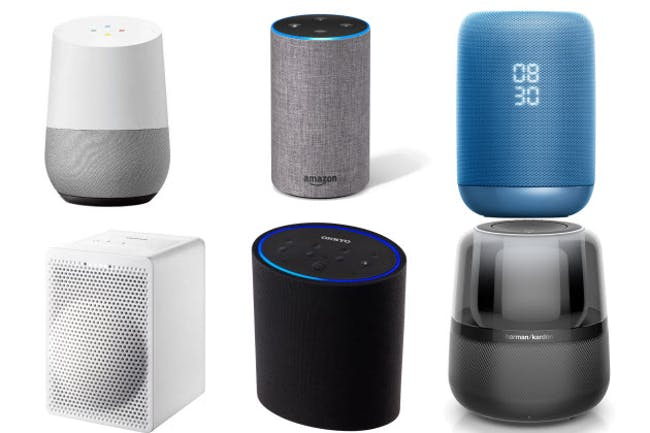
\includegraphics[scale=0.6, clip]{./img/smartspeaker_list.jpg}
        \caption{magentaによるMIDI音楽データ生成までのプロセス}
        \label{fig:magentaによるMIDI音楽データ生成までのプロセス}
    \end{center}
\end{screen}
\end{figure}\\
また囲碁や将棋,チェスなどの競技においても,プロにAIが勝利するなどその精度は以前から高いが,そのAIは一つの競技でしか使用できない特化型人工知能(AGI)でありった.
しかし,英DeepMindが発表したAlphaZeroという様々なボードゲームに対応できる汎用性を持ったAIが発表され,汎用人工知能(GAI)の成長も著しい.\\
自然言語処理を用いた芸術の分野では,2012年にスタートした人工知能を使って小説を生成するプロジェクトが「星新一賞」の第一審査を通過した.
また,絵画や音楽に関してもAIが作成した肖像画が米競売大手クリスティーズのオークションで43万2500ドル(約4900万円)で落札され,AIを用いて新しい作品を作るものが出回っている.\\
 このようにAIの発展は様々な分野においてその成果を上げており,今後は業務の効率化や補助だけにとどまらず,自動車の自動運転や医療の現場でも人間の手よりも高精度なものとして活躍することが期待されている.\\
本研究ではAIによる楽曲生成についての実証実験を行う.
Googole brainによって公開されているTensorflowのライブラリであるMagentaはAI Duetや
そのライブラリを用いて学習データやノード数による楽曲の生成結果の違いを比較,検証し,AIによる楽曲制作が有用なものか調査する.\\
\section{本論文の構成}
本論文の構成は以下の通りである.\\
第1章では本論文の背景と目的について述べている.\\
第2章では本論文で利用する理論について述べている.\\
第3章では実験内容について述べている.\\
第4章では楽曲制作について述べている.\\
第5章ではAIを用いた楽曲制作についての本研究の結論について述べている.\\